
% Straight up stealing preamble from Eli Holmes 
%%%%%%%%%%%%%%%%%%%%%%%%%%%%%%%%%%%%%%START PREAMBLE THAT IS THE SAME FOR ALL EXAMPLES
\documentclass{article}
\usepackage{Sweave}
\usepackage{graphicx}
\usepackage{tabularx}
\usepackage{hyperref}
\usepackage{natbib}
\usepackage{pdflscape}
\usepackage{array}
\usepackage{gensymb}
\usepackage{longtable}
\usepackage{xr}
\usepackage{pdflscape}
\usepackage{amsmath}
 \topmargin -1.5cm        
 \oddsidemargin -0.04cm   
 \evensidemargin -0.04cm  % same as oddsidemargin but for left-hand pages
 \textwidth 16.59cm
 \textheight 21.94cm 
 %\pagestyle{empty}       % Uncomment if don't want page numbers
 \parskip 7.2pt           % sets spacing between paragraphs
 %\renewcommand{\baselinestretch}{1.5} 	% Uncomment for 1.5 spacing between lines
\parindent 0pt% sets leading space for paragraphs
\usepackage{setspace}
%\doublespacing
\usepackage{xr}
%\externaldocument{/Users/aileneettinger/Documents/GitHub/ospree/docs/budburst/budburstms}
%\externaldocument{/Users/aileneettinger/Documents/GitHub/ospree/docs/budburst/budburst_supp} 
 
%%%%%%%%%%%%%%%%%%%%%%%%%%%%%%%%%%%%%%END PREAMBLE THAT IS THE SAME FOR ALL EXAMPLES


%Start of the document
\begin{document}

\pagenumbering{gobble}
\setlength\parindent{0pt}

\title{Response to Reviewers}
\emph{Reviewer comments are in italics.} Author responses are in plain text.\\

\emph{{\bf Referee 1, Comments to the Author}}

\par \emph{The review is a well-written summation of how photoperiod may interact with warming temperatures in limiting or altering the spring phenology of plant species. I enjoyed reading the piece, but for a review in New Phytologist, I found it to be rather short and more narrowly focused on spring leaf out and early spring phenology than was obvious from the title and introduction.}

\par \emph{I would suggest that the authors broaden the scope of the work - while the interplay of photoperiod and temperature in controlling spring phenology is less well studied than the role of photoperiod in dictating senescence, the review would have more impact if it incorporated a section on autumn phenology and how similar shifts in time and space may play out there. I'm not suggesting doubling the length of the review, but some explicit discussion of the implications of Figure 1 on autumn phenology and ecology, as only one example, would be welcome and would give the review a much broader audience. Otherwise, though less desirable, the title and abstract should be revised to be be clearer about the focus on spring leaf out.}
\par We thank the reviewer for the suggestion. We have added several new citations, and sentences on implications for autumn phenology, as well as altering some wording in the introduction. Specifically, we have made the following changes:
\begin{itemize}
\item Line 17: We removed ``spring'' so that the opening sentence of the introduction is broader and now says``Shifts in phenology---i.e., the timing of biological events, including budburst, leafout, and flowering in plants, as well as bird arrival, egg hatching and myriad other biological activities---are some of the most widely documented signals of climate change.''
\item Line 35: We removed ``advances in spring'' to broaden the paragraph. The first sentence now says ``Recent studies suggest that photoperiod cues may eventually restrict phenology in a warmer world.''
\item Lines 62-68: We have restructured this paragraph to explain that the ideas are broadly relevant for diverse species and phenophases. The first sentences of this paragraph now state: ``Our questions are broadly relevant for diverse species and seasonal events. We use a case study of spring woody plant phenology to illustrate several of our points (Boxes 1-2).''  
\item Adding a paragraph on temporal shifts in experienced photoperiod, given observed changes to the timin gof leaf senescence in the fall (Lines XX): ``\par Temporal shifts are likely to yield largers changes in experienced photoperiod for autummn phenology, as well, in temperate areas. Consider again the tree species at latitude 45$^{\circ}$, which may senesence on day of year 300 (October 27), on average (Gill et al 2015), when daylength is 10.5 hours. If senescence shifts 33 days later over the next century (i.e., a rate of 3.3 days per decade, as has been observed, Gill et al 2015), it will experience, at the end of the growing season, a daylength that is 1.3 hours shorter.''
\item Adding the following sentences to Lines XX: ``We have focused here on spring phenology, but future work could also address the sensitivity of model outcomes to shifts experienced photoperiod at the end of the growing season (i.e., autumn phenology). Autumn photoperiod affects photosynthesis, growth, and budset in woody plant species, and photoperiod-induced declines in photosynthetic capacity may constrain carbon sequestration even if warming prolongs leaf senescence (Howe1996, Bauerle et al 2012, Stinziano and Way2017).''

\item Incorporating into our discussion forecasting(Lines XX-XX) the two new references suggested by this reviewer (Bauerle et al 2012 and Stinziano and Way 2017): ``As researchers more fully integrate experienced photoperiod into forecasting, a critical area of further study is understanding \emph{how} photoperiod acts as a cue. Photoperiod seems to interact with temperature to affect phenology \citep[e.g., Box 1,][]{zydlewski2014}; this would explain the divergent effects of photoperiod observed across studies in woody plants (Box 1). However, exactly how it interacts with temperature is not well-defined for most species or populations. For many species, additional experimental and physiological research is necessary, since the dormancy-breaking processes that photoperiod affects require detailed physiological approaches to observe. Though the main ecophysiological processes involved in regulating phenology of woody plants are relatively well-documented, a clear mechanistic understanding of the physiological, molecular, and genetic bases of dormancy are lacking \citep[Box 2][]{hanninen2019, chuine2016}. In addition, photoperiod and temperature cues can differentially affect the phenology of distinct physioslogical processes in woody species, decoupling, for example, responses of growth or leaf development and carbon uptake to warming \citep{bauerle2012,stinziano2017}. Accounting for ecophysiological effects of photoperiod results in quantifiable declines on modeled global gross primary production \citep{bauerle2012}, suggesting that temporal and spatial shifts in experienced photoperiod with climate change may also alter global model estimates.

\end{itemize}
\par \emph{The SI figure could be incorporated into the main text as well. I think it helped drive home the lack of data we have for modeling these responses.}

\par We have moved this figure into the main text.

\par \emph{There is evidence that photoperiod and temperature cues can differentially affect the phenology of different processes in woody species (such as uncoupling of growth or leaf development and carbon uptake [Bauerle et al. 2012 PNAS; Stinziano and Way 2017 PC\&E]). If we incorporate phenological shifts in leaf out into climate models, can we assume that physiological processes are not also impacted separately by photoperiod cues?} 

\par  The reviewer brings up interesting and important points. We have added the recommended citations, which we now  discuss on lines XX-XX:

``Though the main ecophysiological processes involved in regulating spring phenology of woody plants are relatively well understood, a clear mechanistic understanding of the physiological, molecular, and genetic bases of dormancy are lacking \citep[Box 2][]{hanninen2019, chuine2016}. For example, photoperiod and temperature cues can differentially affect the phenology of distinct physioslogical processes in woody species, decoupling responses of growth or leaf development and carbon uptake to warming \citep{bauerle2012,stinziano2017}.''

\par We have also added to the following paragraph (lines XX-XX) to underscore the unanswered questions about how this decoupling will scale up to alter carbon sequestration at the global scale under climate change:
``Understanding the drivers, as well as the consequences, of variation in photoperiod responses across  and within individuals, populations, and species will be critical for forecasting.  What traits are associated with photoperiod sensitivity and does variation in photoperiod sensitivity or related traits have a strong genetic component? If so, are species or populations from some locations or lineages more likely than others to be constrained by photoperiod in their responses to climate change? What are the implications for carbon sequestration under global climate change?''


\par \emph{The figures are nicely designed, but not always adequately described in the legend. For example, in Figure 1, it took me quite a while to work out what each arrow was telling me. In the Figure in Box 2, I can't determine why the background figure is even there - two other figures are covering it, and the one on the bottom left is unclear to me as well - I assume it has the same axes and the background figure? A cleaner version of this, separating out the figures, clearly labeling them and providing a full explanation of the graph in the figure is needed.}

\par We thank the reviewer for pointing out a need for more descriptive figure legends and improved versions of Figure 1 and the figure in Box 2.
For Figure 1, we have modified the figure to make the message clearer. We have also added additional information to the legend.
For the figure in Box 2,  to make the figure more readable we have removed the inset, extended the range of the y-axis, and limited the range of the x-axis (to span the range of photoperiod treatments for most responses). We have also added more detail to the figure legend.


\emph{{\bf Referee 2, Comments to the Author}}
\par \emph{Overall: The review is well written and is presented in a clear and easy to follow structure. I think the inclusion of new analysis should be clearly highlighted.}

\par We thank the reviewer for the time spent reviewing our manuscript. We address the suggestions in detail below. 

\par \emph{Major comments}
\par \emph{Some new analysis and data is included and I think the methods/ datasets should be included in the main manuscript for ease of reading and referencing. Or at least reference the supplementary materials at the points in the text where new analysis is included}
\par We thank the review for suggesting that we need to better reference when new analyses are included in the main manuscript. To address this, we have moved some sections of the supplement to the main text, and for sections that we left in the supplement, we now reference new analyses. Here are places where these changes have been made:
\begin{itemize}
\item We moved the figure that was previously in the supplemental materials to the main text, in Box 1-- now labeled Figure Box 1.2-- where the dataset is described.
\item Lines 73-75, where we now write: ``We use green-up date as an example because it represents an important spring event, signaling the start of the growing season, and global estimates are available.(See ``Quantifying and mapping differences in green-up across the United States and Europe (Figure 2)'' in the \emph{Supplemental Materials} for additional details of this analysis.)"
\item We moved portions of text previously in the Supplemental Materials to the Figure 3 caption, which now says:
``\textbf{A map of experimental photoperiod treatments and their equivalent spatial and temporal shifts} demonstrates that many experiments manipulate photoperiod more dramatically than will occur with climate change. Mapped points (circles and Xes) are locations of experiments in (Wolkovich2019} that manipulated photoperiod (30 total experiments; see Box 1). In 11 out of 30 cases, the difference between experimental treatments exceeded the range in photoperiod experienced across the entire year at the study latitude (Xs; circles mark temporal shifts within a possible range). Note that many studies occur at high latitudes, which experience a wide range of photoperiod across the year. In 13 out of 30 cases, the experimental treatment differences exceeded the photoperiod change that would be experienced with a latitudinal shift of up to 40\degree (shown by lines). See `Mapping temporal and spatial shifts in space and time' in the \emph{Supplemental Materials} for additional details. '' 

\end{itemize}

\par \emph{Minor comments}
\par \emph{-abstract L5. This is a bit misleading as it is a subset of plant species investigated etc. It may be more accurate to describe photoperiod types of response, LD, SD and day-neutral}

\par We thank the reviewer for pointing out the potential for this section to be misleading. We have changed the text to be clear that the summary statistic applies to woody plant spring phenology. The section now says (Line 5): 
"affecting woody plant spring phenology in 84\% of reviewed studies that manipulated photoperiod"
The woody plant spring phenology growth chamber experiments we have read, including those summarized here and others not included in our database, do not clearly define responses as long-day, short day, or day-neutral so we have not summarized them in that way here. 
\par \emph{L120. climate change induced ever earlier springs. Is this correct? What is the data to support it? The statement is made at a global level which may be too broad. Either clarify or provide geographic regions where this is true}
\par We agree that this glosses over the variation in responses across species and geographic areas. We have deleted the phrase. 

\par \emph{L213. A bit more detail could be included here about the current level of molecular/genetic knowledge}
\par We thank the reviewer for pointing out that more detail on the current level of molecular/genetic knowledge would be beneficial. We have added a sentence summarizing the current level of molecular/genetic knowledge and what is needed. The section (Lines 219-221) now says:
``For many species, additional experimental and physiological research is necessary, since the dormancy-breaking processes that photoperiod aeffects require detailed physiological approaches to observe. Though the main ecophysiological processes involved in regulating spring phenology of woody plants are relatively well understood, a clear mechanistic understanding of the physiological, molecular, and genetic basis of dormancy, its release, and the role of photoeriod are lacking  (Hanninen et al., 2019; Chuine et al., 2016, Box 2).''

\par \emph{L222. highlighted more than shown}
\par We now use the word ``highlighted" rather than ``shown," as suggested by the reviewer.

\emph{{\bf Referee 3, Comments to the Author}}
\par \emph{The present manuscript is a review focused on the important topic of the constraint that photoperiod may play in spring phenology dynamics in a warmer world. This is a critical, yet oft overlooked aspect of climate warming impacts on the northern hemisphere. I really appreciated the ideas presented here and think that this review makes an important contribution to this field. I will also note that I jotted down ideas, questions, and comments as I was reading through the paper and repeatedly found that the authors had dealt with these questions or ideas later in the paper! As a consequence, my comments are fairly limited, which is not a function of a surficial review, but rather of a well constructed paper. The writing was clear and logical, making the paper easy to review. Jenn Baltzer}
\par We are grateful for the reviewer's time, positive words, and helpful suggestions.

\par \emph{Line 90: Might this sentence be expanded a bit? Specifically, is there evidence that the potential for northward migrations might be limited by photoperiod constraints? Climate envelope models assume that species will be able shift northward with climate but what if a photoperiod mismatch arises? }
\par We thank the reviewer for this comment. Though we know of no studies documenting photoperiod constraints to range shifts, we did find a recent paper proposing that this might be an increasing concern. We now mention this idea and cite this reference (Lines 90-92 in the revised version):
``For example, poleward shifts in species' ranges cause plants to experience a wider range of daylength throughout the year (Fig. 1), which may pose challenges to organisms undergoing temperature-induced poleward range shifts (Huffeldt 2020). Elevational shifts, in contrast, cause minimal change to the range of daylength throughout the year.''


\par \emph{I really like the comparison presented in figure 1 and described in the paragraph starting on line 97. The example you use in the text is very compelling. }
\par Thank you!
\par \emph{I appreciated and enjoyed the discussion starting on line 142 regarding differential species sensitive to photoperiod having the potential to lead to community-level shifts (i.e., warming favouring those species that are relatively insensitive to photoperiod). I think that these are really neat ideas. A few thoughts/comments here that could be considered in this section: }
\par \emph{- From your knowledge of this literature, do you think that there are commonalities in the taxa that are less or more sensitive to photoperiod? From a plant productivity perspective, for example, might we expect that species compositional shifts associated with photoperiod sensitivity could also results in systematic shifts in ecosystem productivity, or some other systematic difference in ecosystem function? Given that you have already pulled together a database, this could be quite tractable to explore. For example, it would be neat to combine your OSPREE database that a characterizes species photoperiod sensitivity with TRY database has terrific species-level functional trait data to ask questions about whether certain life history strategies also correspond with photoperiod sensitivity. }
\par The reviewer suggests an interesting extension of this work. Indeed, members of our author team are actively working on additional analyses and a separate manuscript that explores the extent to which functional traits from the TRY database correspond to photoperiod sensitivity, as well as sensitivity to forcing and chilling, estimated from our database. In our revised manuscript, we mention this research question on lines 216-218, where we write:
``Understanding the drivers, as well as the consequences, of variation in photoperiod responses across species and populations will be particularly benecial for forecasting. For example, what traits are associated with photoperiod sensitivity and does variation in photoperiod sensitivity or related traits have a strong genetic component? If so, are species or populations from some locations or lineages more likely than others to be constrained by photoperiod in their responses to climate change?''

 \par \emph{- What about across latitudes? You mention ecotypic divergence in an earlier section in the paper but seems to me that this ecotypic divergence could alter these competitive outcomes as well. For example, aa PhD student of mine conducted a common garden study with black spruce collected across a 2000 km latitudinal gradient (Sniderhan et al. 2018); we grew all trees at a common photoperiod and the high latitude populations would produce a single whorl of growth and then harden off while the more southerly populations just kept on growing until we forced them into a winter. This was not a photoperiod study but this suggests to me that there could be variation across species ranges in their responsiveness to photoperiod that could alter how community dynamics play out under warming.}
\par The reviewer highlights an interesting and important point- there can be variation in photoperiod sensitivity across latitude. We now cite a reference we read after reading the article mentioned by the reviewer (Johnsen and Seiler 1996, referenced in Sniderhan et al. 2018). In our revised manuscript, we mention variation in photoperiod sensitivity across latitude in lines 128-132, where we write `A challenge in predicting if or when the trend of earlier phenology with warming may slow or stop abruptly is the wide range of observed photoperiod sensitivity (see Glossary) across species (Flynn and Wolkovich, 2018; Zohner et al., 2016; Sanz-Perez et al., 2009), latitudes (Ettinger et al 2020, Partanen et al., 2005, Johnsen and Seiler 1996), populations (Gauzere et al., 2017; Saikkonen et al., 2012; Caffarra et al., 2011b; Bradshaw and Holzapfel, 2007; Vihera-Aarnio et al., 2006), and ecotypes (Howe et al., 1995).

\par \emph{- Line 38 reads: ``and the trend of ever-earlier springs with warming may halt." This assumes that all species are responsive to both temperature and photoperiod cues. If the species differences in responsiveness that you describe there are at play, might this mean that such a halting would not occur? In other words, we might expect certain plant taxa to keep up this trend while others don't? }
\par We agree that this glosses over the species differences we describe and have deleted the phrase. 
\par \emph{You have made beautiful figures that really clearly articulated the problem at hand. A few comments/suggestions: }
\par \emph{1. In Figure 1, you show two shifts for the higher latitude location (early season and peak season) but only one for the lower latitude location. I think it would be useful to show and talk about shifts for both. This would highlight the fact that early season shifts correspond to different relative poleward shifts depending on the latitude. While these differences are apparent at mid-growing season, they would be exaggerated in early season. You may have made this point in the text and I missed it (if so, sorry) but highlighting the fact that warming at higher altitudes results in much more extreme changes in day length is worthwhile given that it is at exactly those latitudes that warming is happening most rapidly. }
\par We thank the reviewer for these suggestions. We have modified Figure 1, as suggested by the reviewer, and have added substantial text to the figure caption to make it stand alone. The figure legend now says:
``Temporal (i.e., phenological) shifts in activity yield larger changes in experienced photoperiod compared to spatial (i.e., latitudinal) shifts} on the same day of year, due to patterns in photoperiod variation with latitude and by day of year. Here, we show this variation at two latitudes (22.5\degree, 45\degree), using hypothetical spatial and temporal shifts. These shifts are based on observed rates with recent global warming: for spatial shifts, 6-17 kilometers per decade, or approximately 0.5-1.5\degree in 100 years (Parmesan \& Yohe 2003, Parmesan 2006); for temporal shifts, 2-3 days per decade, or 30 days in 100 years (Parmesan 2006, Chen et al 2011). These potential, plausible shifts highlight the greater magnitude in daylength changes from temporal shifts in the early spring, close to the vernal equinox (e.g., day of year 91), versus close to the summer solstice (e.g., day of year 182) at temperate latitudes.  It is also apparent that early spring temporal shifts at high latitudes results in more extreme changes in daylength than shifts at lower latitudes (e.g., a temporal shift 30 days earlier results in a reduction in daylength of 94.5 minutes at 45\degree versus 39.5 minutes at 22.5\degree).''

\par \emph{2. In Figure 2, it would be really cool to have a fourth panel: specifically, a trend map for the period between 2009 and 2012 (akin to what is done with NDVI data). Although this figure exemplifies the ideas that are needed for the figure, I think for a review paper that those global trends would be nice to include as well. A short sentence could be added to line 86 to show the magnitude of the trends. }
\par We thank the reviewer for sharing these ideas!  We were intrigued by the reviewer's suggestion to quantify photoperiod trends. Below, we include a modified figure that incorporates this. We quantified the trend across 2009-2018 in panel C. Note that in many areas, trends were highly variable (panel D shows standard deviation of these trends), with wide uncertainty intervals. We decided not to include these additional panels in our revised manuscript because this variability makes the trends difficult to interpret and draw conclusions about. It may be that this time period is not sufficient to identify strong trends in shifts of photoperiod at green-up, given the annual variation in photoperiod at green-up (i.e., panels A,B).
\par
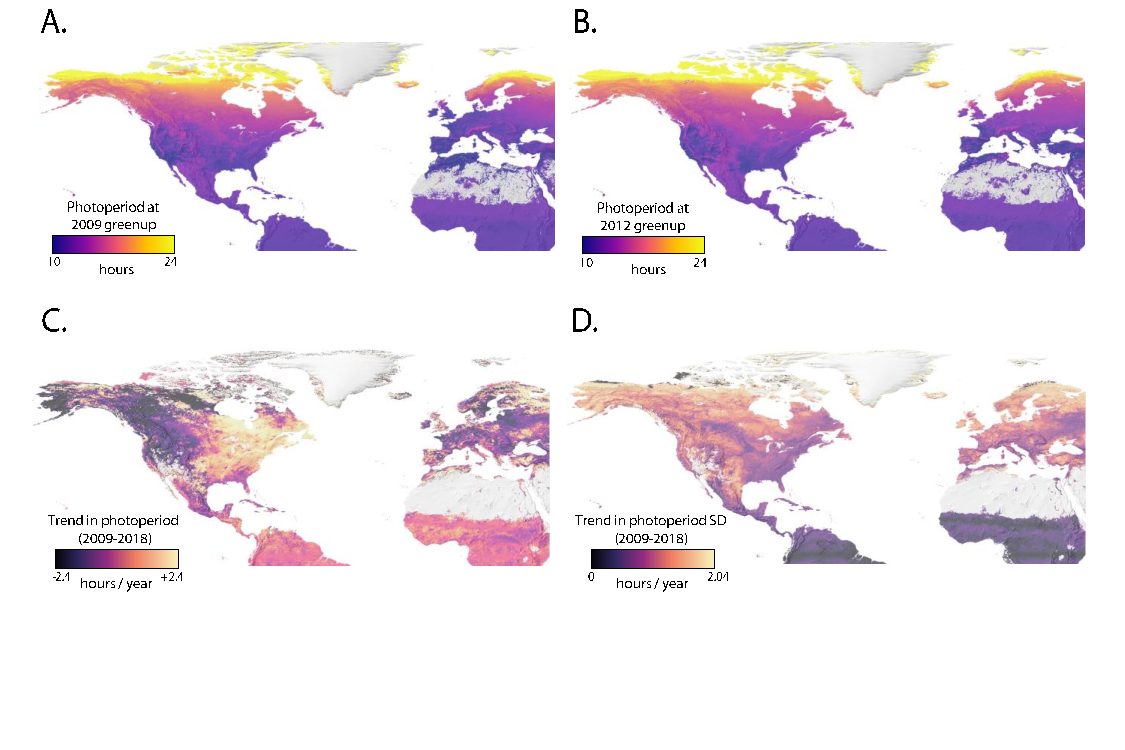
\includegraphics{../figures/Greenup_corr_sm_leg_4panels_sds.pdf} %

\par \emph{3. In my opinion, figure 3 loses impact and interest because it is not stand alone. The reader is required to bounce back and a forth between the paper and the supplement to interpret this figure. I would suggest that the figure caption should be expanded to make the figure stand alone. }
\par We thank the reviewer for these suggestions, and have added substantial text to the figure caption to make it stand alone. The figure legend now says:
``\textbf{A map of experimental photoperiod treatments and their equivalent spatial and temporal shifts} demonstrates that many experiments manipulate photoperiod more dramatically than will occur with climate change. Mapped points (circles and Xes) are locations of experiments in (Wolkovich2019} that manipulated photoperiod (30 total experiments; see Box 1). In 11 out of 30 cases, the difference between experimental treatments exceeded the range in photoperiod experienced across the entire year at the study latitude (Xs; circles mark temporal shifts within a possible range). Note that many studies occur at high latitudes, which experience a wide range of photoperiod across the year. In 13 out of 30 cases, the experimental treatment differences exceeded the photoperiod change that would be experienced with a latitudinal shift of up to 40\degree (shown by lines). See `Mapping temporal and spatial shifts in space and time' in the Supplemental Materials for additional details. '' 

\par \emph{4. I really like figure 4. }
\par Thank you!
\par \emph{5. I found the boxes useful additional information. I appreciated the species-specific detail in box 1 that supported the ideas in the main text and box 2 highlights the potential advances in this field that a could be achieved with molecular tools.}
\par We thank the reviewer for these positive comments!
%%%%%%%%%%%%%%%%%%%%%%%%%%%%%%%%%%%%%%%%
\end{document}
%%%%%%%%%%%%%%%%%%%%%%%%%%%%%%%%%%%%%%%%
